\documentclass{article}

% \usepackage[spanish]{babel}

\usepackage[utf8]{inputenc}
\usepackage{graphicx}
\usepackage{amsfonts}
\usepackage{amsmath}

\title{Ecuaciones en diferencias}

\author{Alumnos de 3er semestre grupo 2}

\date{18 de septiembre de 2017}

\begin{document}

\maketitle

Si en una ecuación en diferencias, la función f no depende de n, la ecuación en diferencias es autónoma. $\mathbb{R}$.

\section{Ecuaciones de primer orden}

\subsection{Ecuaciones lineales}

Una ecuación lineal en diferencias de primer orden tiene la forma $x_{n+1}=ax_n$ donde $a$ es una constante. 

La fórmula para resolver ecuaciones lineales es:
\begin{equation}
  \label{lineal}
  x_n=a^nx_0
\end{equation}

Por ejemplo, si inciamos una inversión con 1000 pesos con un interés mensual del 1\%, obtenemos lo siguiente:

\begin{center}
  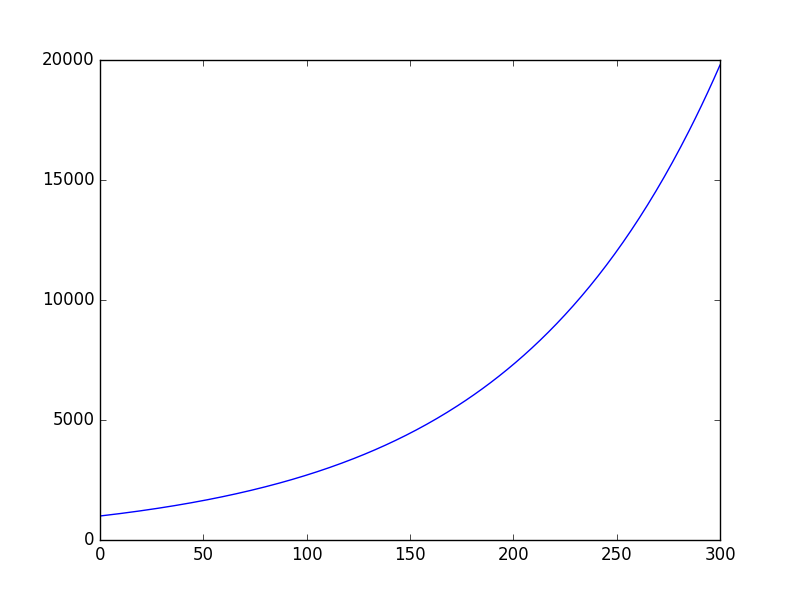
\includegraphics[width=8cm]{inversion.png}
\end{center}


$x_{n+1}=1.01x_t$

Estas ecuaciones hacen que una ecuación que inicialmente era de esta manera $x_{n+1}=x_n+2(x_n)$ puede escribirse de manera que la ecuación solo dependa de $x_n$ y queda de la siguiente forma:

$x_n=3^n(4)$0     


\subsection{Ecuaciones afines}

Una ecuación afín en diferencias de primer orden tiene la forma $x_{n+1}=ax_n+b$ donde $a$ es una constante. 

\begin{equation}
  \label{afin}
  x_n=a^n(x_0-\alpha)+\alpha
\end{equation}

donde $\alpha=\frac{b}{1-a}$. 

Para deducir esta fórmula usamos que $$\sum_{i=0}^{n-1}a^i=\frac{a^n-1}{a-1}$$.

\subsection{Ejemplito}

Nuestro compañerito Pepe muere en raras circunstancias (después de tener su examen de Álgebra II), luego descubren lo radiante de su ser. cada 20 años el elemento radioactivo decae a razón de $2\%$, si inicialmente contenía 2 kilitos de puro amor ¿Cuánto tendrá cuando se vea un poco más feo (como quien digo, dentro de 200 años)?

\subsection{Un ejemplito más}

(esto continuará, no lo pude hacer completo)


\section{Ecuaciones de segundo orden}

El método para resolver estas ecuaciones está inspirado en la fórmula \ref{lineal}.

Para resolver una ecuación en diferencias de segundo orden se usa la ecuación resolvente.

Una ecuación en diferencias de segundo orden , tiene la forma $a_{k+2}=f(a_k ,a_{k+2}$
Esta ecuaci\'on no tiene raices reales $$x^2+1=0$$

\subsection{Ejemplo 2}

Se plantea la siguiente ecuacción en diferencias:

$a_{n+2}=2a_{n+1}-a_{n}$ con condiciones iniciales : $a_{0}=4 ; a_{1}=7$

Solución:

Primero igualamos la ecuación en diferencias a cero:

$a_{n+2}-2a_{n+1}+a_{n}=0$ Esto último nos genera una ecuacción resolvente que se factoriza y resuelve facilmente:

$r^2-2r+1=0$

${(r-1)^2=0}$

${r=1}$
La solución general a esta eccuación en diferencias seria:

$a_{n}=\lambda_{1}(1)^n+n\lambda_{2}(1)^n$

Sin embargo, el problema nos da condiciones iniciales específicas.Entonces procedemos a plantear un sistema de ecuaciones para poder satisfacer las condiciones iniciales.

$a_{0}=4=\lambda_{1}(1)^0+0\lambda_{2}(1)^0$

$a_{1}=7=\lambda_{1}(1)^1+1\lambda_{2}(1)^1$

Al resolver lo anterior obtenemos los siguientes valores:

$\lambda_{1}=4 y \lambda_{2}=3$

Con lo que la solución final sera:

$a_{n}=4(1)^n+3n(1)^n$
\subsection{Números  complejos}

Un complejo es un número de la forma $z=a+bi$, $a,b\in\mathbb{R}$ , con $i^2=(-1)$, a parte real, b parte imaginaria.

El módulo de un número complejo: $|a+bi|=\surd(a^2+b^2)$.


El argumento de un número complejo es el ángulo comprendido en(continuará)


\subsection{Ejemplo}

Para cada $n$, considera el determinante $n\times n$ dado por:
\begin{equation}
  \label{eq:1}
  D_n=\det
  \begin{pmatrix}
    b & b\\
    b & b 
  \end{pmatrix}
\end{equation}




\end{document}

